\chapter{Measurements}
\section{Dimensional metrology}
	The \de{dimensional metrology} is the study of geometrical measurements (such lengths, areas, roughness). The \textbf{confidence} in the dimensions of this measurement systems is critical for their operation and establishes an agreement between the vendor and the customer on the quality being traded.
	
\subsection*{Length standards}
	A \textbf{measurement standard} is a practical realization of the definition of a measurement unit. As example the first international standard of length was a platinum-iridium bar names \textit{International Prototype Metre}; now the definition is changed and a meter is the length of the path travelled by the light in a vacuum in $1/299\,792\,458s $ (and so it's now a derived unit).
	
	The idea of standard allows the definition of the traceability chains (usually consisting of 4 levels) that's transferred between levels using calibration.
	
	\begin{SCfigure}[1][bht]
		\centering 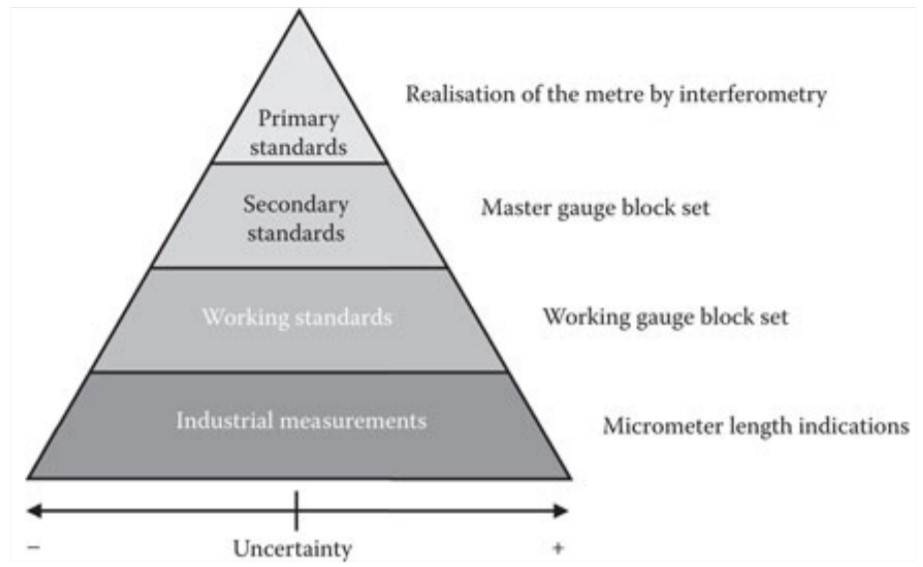
\includegraphics[width=7cm]{trace-levels}
		\caption{pyramid representing the 4 levels of traceability chain.}
	\end{SCfigure}
	
	A length standard can consist of a edge gauges block of, more easily, using \textbf{line standard} which provide the reference lengths as the distance between two parallel lines on the surface of the object (so, as example, a simple ruler or calliper). The line standard is often used for calibrating the scales of optical vision system.
	
	\begin{SCfigure}[2][bht]
		\centering 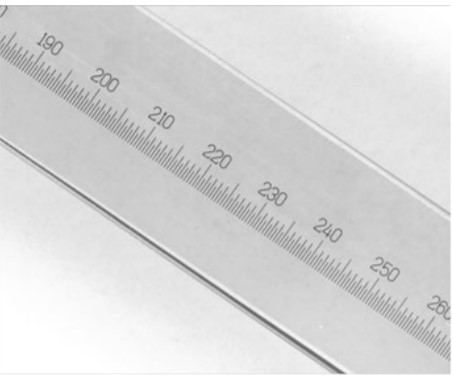
\includegraphics[width=4cm]{ruler}
		\caption{example of a line length standard.}
	\end{SCfigure}
	
\subsection{Displacement sensors} 
	The contact displacement sensor measure the linear position of an object by physically contacting its surface with a prove. An example of digital comparator of displacement is the \textbf{LVDT} (\textit{Linear Variable Differential Transformer}) transducer. In this case the displacement is related to the motion of a movable electromagnetic core that determines a change of mutual inductance between the primary and secondary coils that's then measured by a voltmeter.
	
	\begin{SCfigure}[2][bht]
		\centering 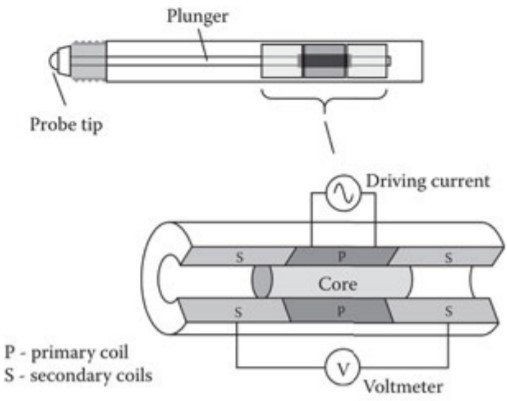
\includegraphics[width=4cm]{lvdt}
		\caption{functional schematic of an LVDT displacement sensor.}
	\end{SCfigure}
	
	Displacement can also be measured using \textbf{encoders} that determines a (relative or absolute) position in digital format by counting the number of optical/magnetic/inductive pulses. \\
	Relative encoder are easier to implement and requires only two tracks to measure the displacement and it's direction, but every time it's necessary to restart from a known position. Considering instead an absolute encoder the minimum number of tracks to measure a length $l$ with a resolution $r$ is $\lceil \log_2 (l/2) \rceil $ (for example to measure a length of $l=1m$ with a resolution of $r=1\mu m$ the minimum number of tracks is 20); this measure relates also to the number of bits representing the measure.
	
	In general absolute encoders don't presents masks with a binary encoding, but they use the \textit{Gray code} (in order to avoid the problem of multiple wrong reads of the sensor while being near to the commutation stage) that assures only one change of bit for each step.
	
	\begin{SCfigure}[1][bht]
		\centering 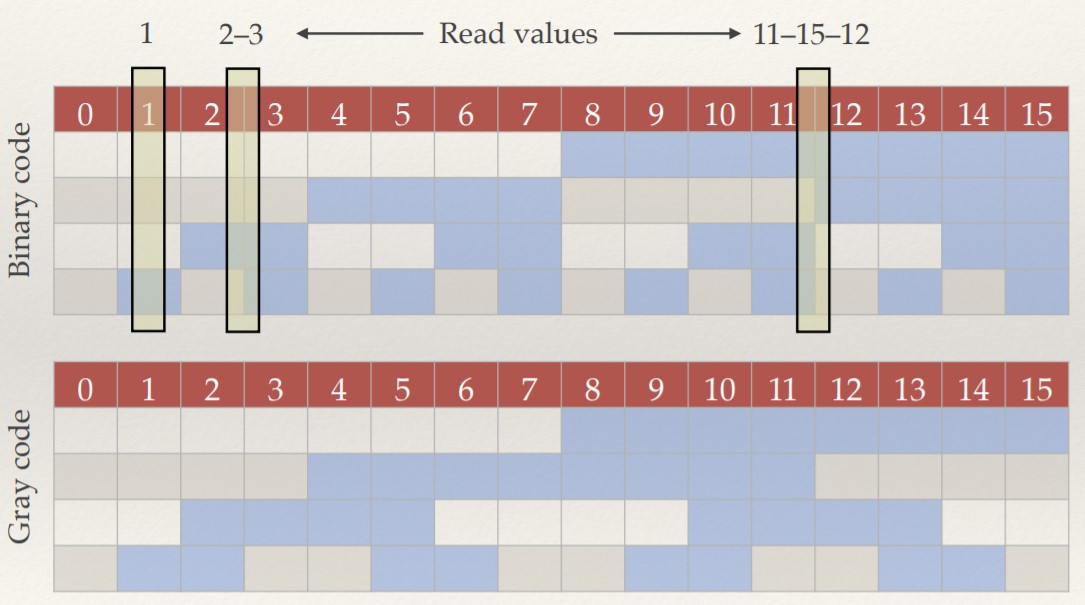
\includegraphics[width=8cm]{greycode}
		\caption{binary code vs Gray code masks for absolute encoders.}
	\end{SCfigure}
	
	\paragraph{Non-contact displacement sensors} The previous explained measurement method for displacement require a contact between the system and the object to be probed, but it possible to create systems contact free using the following measurement principles:
	\begin{itemize}
		\item \textbf{light interferometry}: in this case the system  consists of a laser source that splitted by a beam into two retroreflectors (as shown in figure \ref{fig:meas:interferometer}).		
		
		\begin{SCfigure}[1][bht]
			\centering 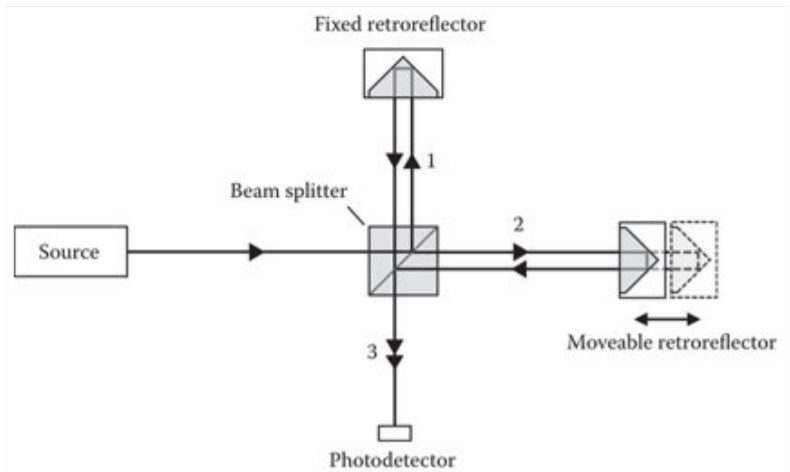
\includegraphics[width=6cm]{las-sys}
			\caption{schematic representation of a laser interferometer.} \label{fig:meas:interferometer}
		\end{SCfigure}
		 
		 The intensity of the interference signal is function of the phase difference between the superimposed beams ($0^\circ$ for constructive interference, $180^\circ$ for the destructive one). The intensity of the interference signal repeats with displacements of the retroreflector equal to one half of the wavelength $\lambda$ of the light beam and, by interpolation of the phase within a fringe period, it's possible to achieve sub-nanometre resolutions. In general the resolution is great ($10nm$) with a range up to hundreds of meters (and so it has a huge dynamic range);
		 
		 \item \textbf{light intensity}: this system has an high resolution but a limited range  and uses fiber optics carrier to enlight the surface and measure the reflected light;
		 \begin{figure}[bht]
		 	\centering 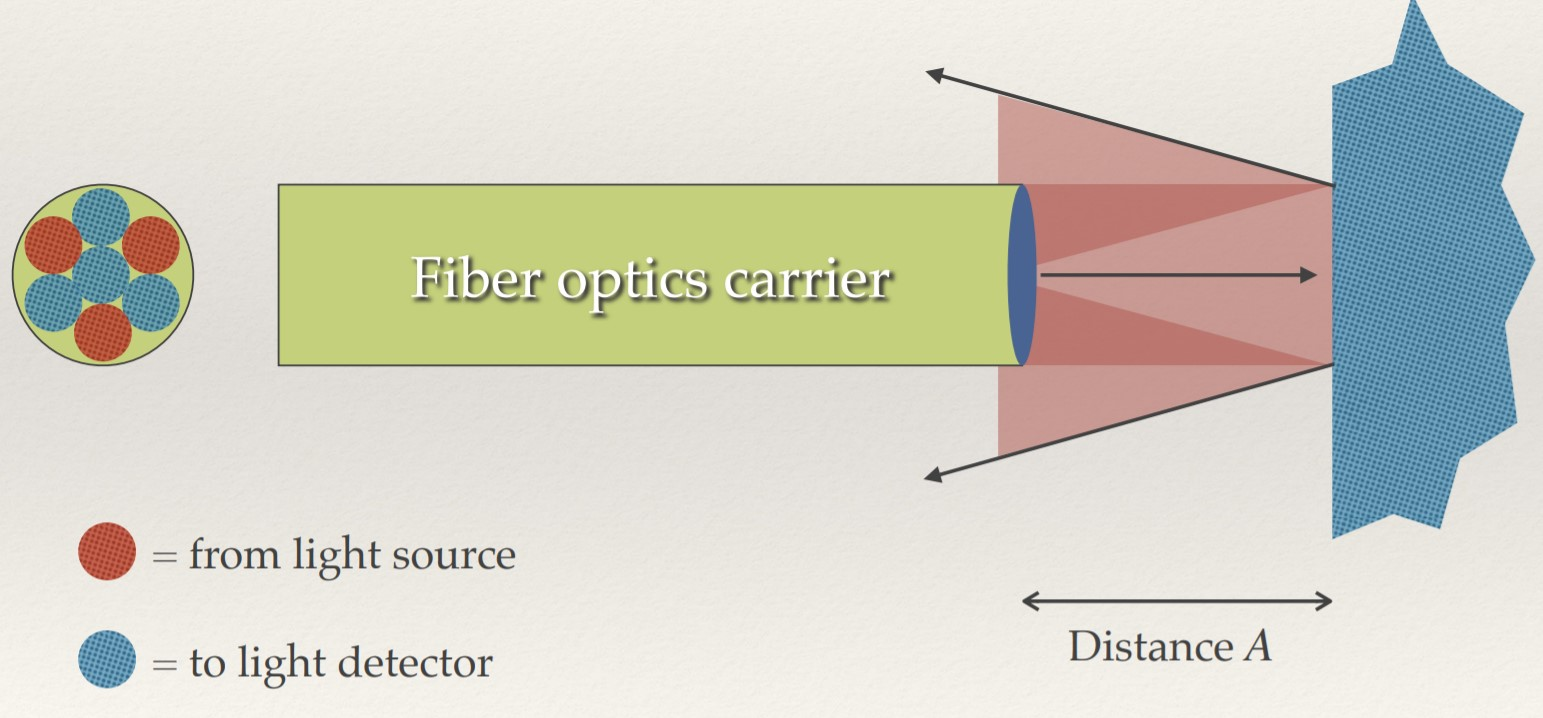
\includegraphics[width=7cm]{fibermeasure}
		 	\caption{schematic representation of a light intensity measurement system.}
		 \end{figure}
	 
	 	\item \textbf{trilateration}: in this case we use a line pixel array to detect the shift of the reflected light source.
	 	
	 	\begin{SCfigure}[1][bht]
	 		\centering 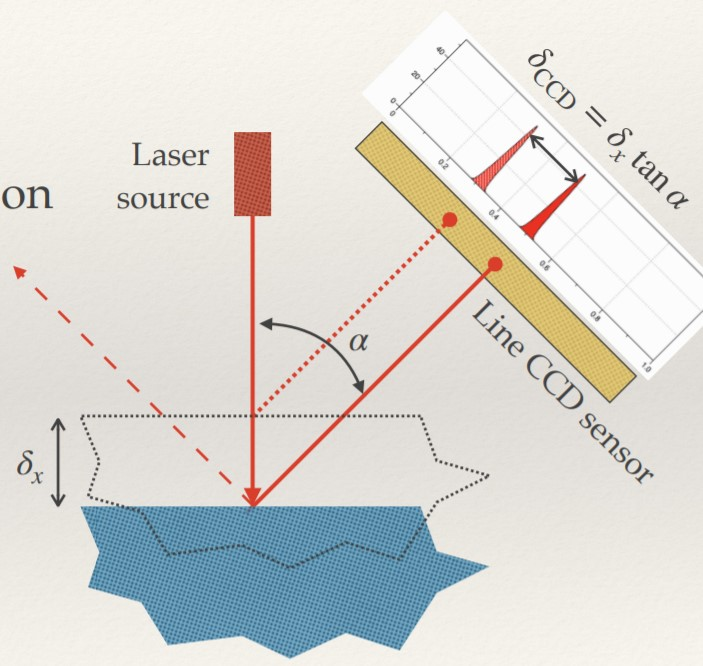
\includegraphics[width=5cm]{trilateral}
	 		\caption{schematic representation of a trilateration measurement system.}
	 	\end{SCfigure}		
	\end{itemize}
	
\subsection{Form measurement}
	\paragraph{Straightness and roundness} The \de{straightness} is measured as lateral deviation along a displacement; in this case the reference line can be computed by interpolation (by computing as example the least-square line). With an analyses of the surface we can define the parameters such the peak-ref deviation $STR_p$, the valley-ref deviation $STR_v$, the peak-valley deviation $STR_t = STR_p + STR_v$ and the RMS deviation $STR_q$.
	
	\begin{SCfigure}[2][bht]
		\centering 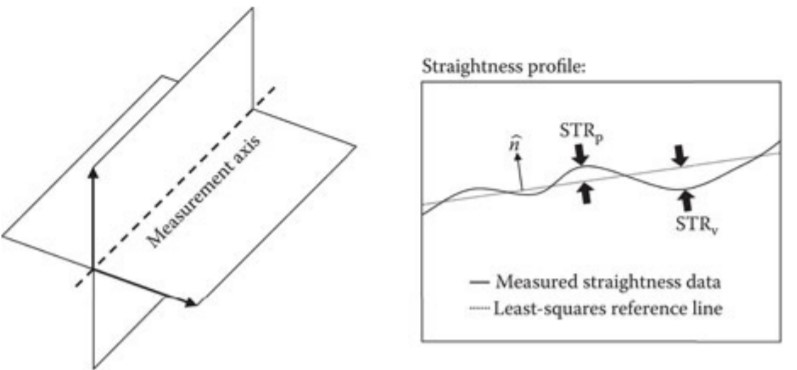
\includegraphics[width=6cm]{straightness}
		\caption{measurement axis and straightness profile with main parameter of this kind of form measure.}
	\end{SCfigure}
	
	Similarly we can define the same parameters for a circular surface determining so the \de{roundness} $RON$ of the piece.
	
	\textbf{Flatness} can be regarded as the straightness in two dimension (on a surface, not a axis), while \textbf{parallelism} defines a tolerance zone respect to a datum, rather than respect to the reference line.
	
	\begin{SCfigure}[2][bht]
		\centering 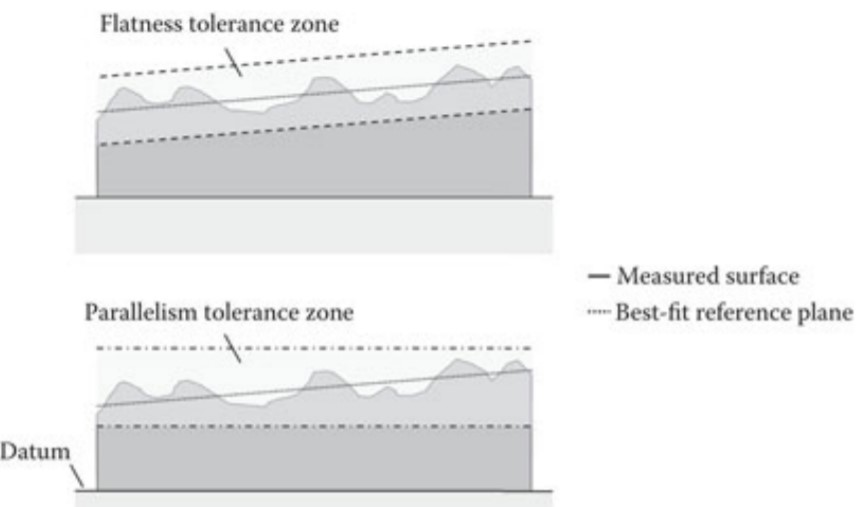
\includegraphics[width=8cm]{flat-par}
		\caption{flatness and parallel zone tolerance for a piece.}
	\end{SCfigure}
	
	In order to asses the flatness we can use an optical flat that use the patterns of the fringes due to light interferometry to determine the flatness of the surface.
	
	\begin{SCfigure}[2][bht]
		\centering 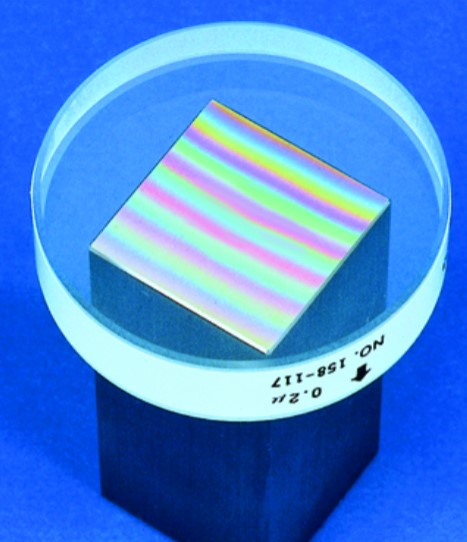
\includegraphics[width=3cm]{opt-flat}
		\caption{example of an optical flat system to measure flatness.}
	\end{SCfigure}
	
	\paragraph{Roughness} To determine the \de{surface roughness} of a surface we need to split it's topography (all wavelength) into surface texture (short wavelength) and  surface form (long wavelength associated to the baseline). In particular the roughness is a one dimensional texture measured along a single scan line.
	
	\begin{SCfigure}[2][bht]
		\centering 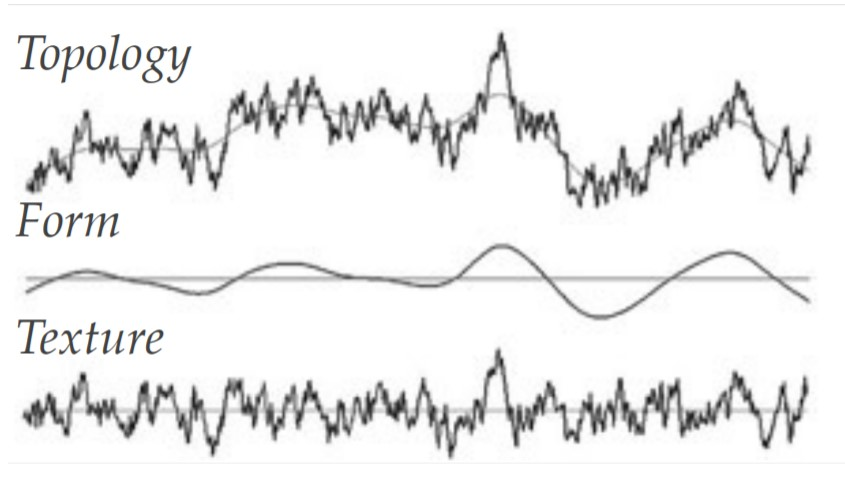
\includegraphics[width=5cm]{rough-top}
		\caption{topology, form and texture surface for a piecea.}
	\end{SCfigure}

	Texture measure can be either be contact (stylus sliding orthogonally to the surface) or contact-less (optical analysis that's intrinsically bi-dimensional). In general non contact texture instruments provides a height map image of the surface that can be easily analysed and can convey a lot of information. In general non contact texture instruments have a limitation in the resolution $r$ (compared to the contact one) that depends on the numerical aperture $A_n = n \sin\alpha$ following the relation $r = k \lambda /A_n$ (where $k=0.61$ is the Raylight criterion,$\lambda$ is the light wavelength and $n$ is the refractive index of the optic).
	
	In general to compute the parameter $Ra$ associated to the \textbf{surface roughness} we consider the equation
	\begin{equation}
		Ra = \frac 1 L \int_0^L |z(x)| \, dx
	\end{equation}
	where $L$ is the reference length on which we compute the parameter and $z(x)$ represent the deviation of the surface from the centre line.
	
	\paragraph{Reversal principle} A simple way to separate error is to use the \de{reversal principle} that consist on a double measure reversing the measurement system.
	
	\begin{SCfigure}[2][bht]
		\centering 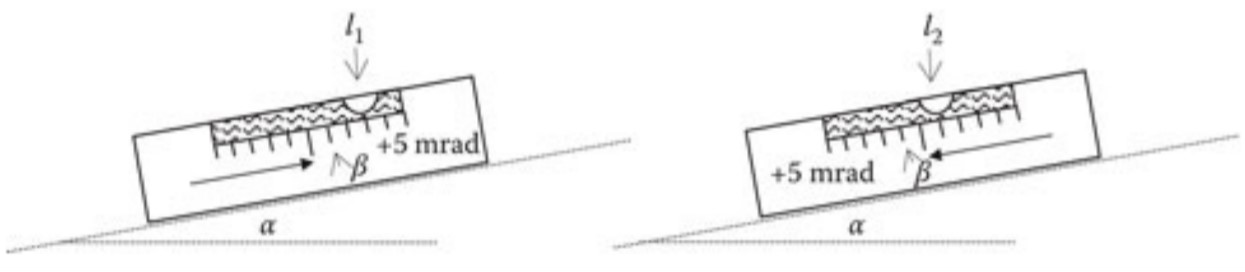
\includegraphics[width=7cm]{rev-princ}
		\caption{application on where the reversal principle can be useful.}
		\label{fig:meas:reversal}
	\end{SCfigure}
	
	Let's consider the practical case shown in figure \ref{fig:meas:reversal} of the instrument shown that allows to compute the angle $\alpha$ of the inclined plane on which is placed by transducing the rotation in the displacement $l$. If the measurement system present an imperfection that translates to an addition of the angle $\beta$ to the measure, this offset error can be compensated using the reversal principle.\\
	Knowing that the first measure gives a displacement $l_1 = \alpha + \beta$, by reversing the orientation of the instrument the output becomes $l_2 = \alpha - \beta$: this allows to calculate more precisely the value $\alpha$ and the error $\beta$ introduced by the system as
	\[ \alpha = \frac{l_1 + l_2}{2} \qquad \ \qquad \beta = \frac{l_1-l_2}{2} \]
	Once that the error $\beta$ is computed and known there's no need to perform this operation every time we want to do a measure.

\section{Statistics and uncertainty}
	The graphical and mathematical techniques that allow to describe the behaviour of a stochastic variable are called \textbf{descriptive statistics}. In this analysis it's important to define the \de{population} as the entire set (that can be both finite or infinite) of all possible observation and the \de{sample} as a random subset drawn from a population.  A sample can be extracted
	\begin{itemize}
		\item with re-insertion, used for the \textbf{simple random sampling}, where each extract element is returned to the population (and so a re-extraction might occur). This process is good when the number $n$ of samples is way less than the size $N$ of the population;
		
		\item without re-insertion, used for the \textbf{bulk sampling}, where each extracted element reduces the remaining population and so this process is suggested when $n\simeq N$.
	\end{itemize}
	
	\paragraph{Frequency and probability} We define the \de{frequency} of a random variable as the number of times a given value is observed for a certain number of observation; from that we can define the \de{probability} as the ratio of the frequency respect the total number of observation. 
	
	When the random variable is discrete ($x\in \mathds I$) then both frequency and probability can be easily calculated, while when the variable is real evaluated ($x\in \mathds R$) we have to introduce the concept of \textbf{classes} (or bins), a set of contiguous intervals of known width (not necessary with the same width); with this definition we can define the probability as the ratio between the observation in a certain class over the whole number of observations; we can also define the \textbf{probability density} as the probability of a class divided by it's bin width. The number $n$ of bins can be computed considering the following binning formulas: 
	\begin{equation}
	\begin{aligned}
		\textrm{Scott:}& \qquad n = 3.5 s_x N^{-1/3} \\ 
		\textrm{Sturges:}& \qquad n = \big\lceil 1 + \log_2(N) \big\rceil
	\end{aligned}
	\end{equation}
	where $s_x$ is the standard deviation (that will be described later) of the sample. 

	In order to analyse frequencies/probabilities we can use graphical instruments like histograms in which the vertical axis can describe the frequency, the frequency density, the probability and the probability density.
	
	\begin{SCfigure}[1][bht]
		\centering 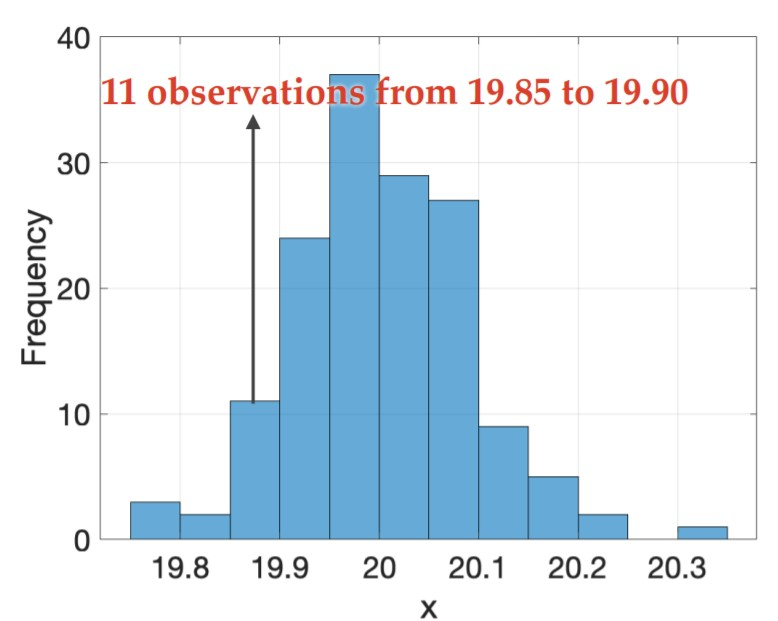
\includegraphics[width=5cm]{histo}
		\caption{example of a histogram display the frequency of a real evaluated random variable.}
	\end{SCfigure}

\subsection{Estimators}
	\paragraph{Central tendency estimators} The \de{central tendency estimators} are used to compute the \textit{central value} of a sample/population; the first main central tendency estimator is the \de{mean} operator that's usually written as $\mu$ for population and $\overline x$ for a sample $x$ and it's defined as
	\begin{equation}
		\mu = \sum_{i=1}^n x_i f(x_i) \qquad \qquad \qquad \qquad \overline x = \sum_{i=1}^n \frac{x_i}{n}
	\end{equation}
	where $x_i$ is the value associated to the $i$-th observation (in the case of the sample mean, but equally it relates to the population). Another central estimator is the \textbf{median} defined as
	\begin{equation}
		\textrm{Med}(x) = \begin{cases}
			\dfrac{x\left(\frac n2\right) + x\left(\frac{n+1}{2}\right) }{2} \qquad & \textrm{when $n$ is even} \\
			x\left(\frac{n+1}{2}\right) \qquad & \textrm{when $n$ is odd}
		\end{cases}
	\end{equation} 
	
	As last operator we define the \textbf{mode} as the most frequent value.
	
	\paragraph{Dispersion estimators} \de{Dispersion estimators} can be used to compute \textit{how away} is spread a random variable respect to the central value. The first operator is the \de{range} that determines the width of the bin associated to a value $x_i$:
	\begin{equation}
		\textrm{rng}(x_i) = \max(x_i) - \min(x_i)
	\end{equation}
	
	A more important operator is the \de{variance} ($\sigma^2$ for population, $s^2$ for sample) that can be calculated by firstly determining the mean of the sample:
	\begin{equation}
		\sigma^2 = \frac{\sum_{i=1}^n (x_i-\mu)^2 }{n} \qquad \qquad \qquad \qquad s^2 = \frac{\sum_{i=1}^n (x_i-\overline x)^2 }{n-1}
	\end{equation}
	The \de{standard deviation} is simply the square root of the variance.
	
\subsection{Probability distributions}
	Using cumulative histograms of a population it's possible to calculate the probability of finding a value in a given range $[a,b]$ as
	\[ P(a<x<b) = f_{cd,l}(b)-f_{cd,l}(a) \]
	where so $f_{cd,l}(\cdot)$ is the \textbf{cumulative probability density function}. The problem of this relation is that the population is rarely known and the \textit{shape} (in statistical expression, the \textbf{distribution}) of the histogram can be different for different variables.
	
	Defining reference distributions in mathematical terms allows to calculate probabilities without knowing the entire population. Reference distribution are identified for both discrete and continuous random variables. In this section we will discuss only the real evaluated probability distribution because they relate better to measuring systems.
	
	\paragraph{Continuous distribution} Given a continuous random variable $x\in\mathds R$, knowing it's \de{probability density function} PDF $f_{pd}(x)$ we can compute the probability of having a value in the range $[a,b]$ as
	\begin{equation}
		p(a<x<b) = \int_a^b f_{pd}(x)\, dx
	\end{equation}
	Using cumulative distributions we can determine the \de{cumulative density function} CDF both lower tail $f_{cd,l}$ and upper tail $f_{cd,u}$ as
	\begin{equation}
	\begin{aligned}
		f_{cd,l}(x) & = \int_{-\infty}^x f_{pd}(\xi)\, d\xi \\
		f_{cd,y}(x) & = \int_x^\infty f_{pd}(\xi)\, d\xi = 1 - f_{cd,l}(x) \\
		\Rightarrow \qquad p(a<x<b) &= f_{cd,l}(b)-f_{cd,l}(a)
	\end{aligned}
	\end{equation}
	From this last equation we can see that the probability of having a precise value $x_0\in x$ in a real  evaluated random variable is always zero ($P(x=x_0) = 0$).
	
	\paragraph{Uniform distribution} The simplest continuous distribution is the \de{uniform} one that's characterized by just 2 parameters, the two bound $a$ and $b$ of the distribution. We mathematically describe a random variable $y$ as uniformly distributed in the interval $[a,b]$ by writing
	\[ y \backsim \mathcal U(a,b) \]
	where
	\begin{equation}
		f_{pd}(y) = \begin{cases}
			\dfrac{1}{b-a} \qquad& a \leq y \leq b \\0 & \textrm{otherwise}
		\end{cases}
	\end{equation}
	
	\paragraph{Normal distribution} The \de{normal distribution} is one of the most used relations and it's characterized by a mean value $\mu$ and a variance $\sigma^2$. We can define the normal distribution as
	\begin{equation}
	\begin{aligned}
		y &\backsim \mathcal N(\mu,\sigma^2) \\
		f_{pd}(y) &= \frac 1 {\sigma \sqrt{2\pi}} e ^{-\frac 1 2 \left(\frac{y-\mu}{\sigma}\right)^2}
	\end{aligned}
	\end{equation}
	We can observe that the distribution computed as $\frac{y-\mu}{\sigma}$ behaves as a normal distribution with zero mean and unit variance:
	\[ \frac{y-\mu}{\sigma} \backsim \mathcal N(0,1) \]
	
	\paragraph{Chi-square distribution} The \de{chi-square} distribution of order $k$ is a sum of $k$ 
	
	
	
	
	
	
	
	
	
	
	
	
	
	
	
	
	
	
	
	
	
	
	
	
	
	
	
	
	
	
	
	
	